\chapter{Theoretical Background}
\label{ch:theory}

This chapter attends to the theoretical background of the technologies used in this thesis.

\section{Word Representations}

While it is trivial to use images as input for machine learning techniques, this is not the case for language. Images already come in matrix form while words appear as discrete objects. Before language can be used for machine learning, words have to be transformed into a matrix first. A function $W(\text{word}) \rightarrow \mathbb{R}^n \quad \text{word} \in V$  which encodes words from a vocabulary $V$ into a $n$-dimensional matrix is called a word embedding.
\medskip

The easiest way to achieve this is a one-hot encoding of a vocabulary. We take the vocabulary which is a list of $N$ words and label the words sequentially. A word vector is created by getting the index of the word from the vocabulary and setting the value of the word vector at the word-index to one and all other entries to zero.

\begin{equation*}
    \begin{aligned}
        W(\text{"dog"}) = [1, 0, 0] \\
        W(\text{"cat"}) = [0, 1, 0] \\
        W(\text{"bee"}) = [0, 0, 1] \\
    \end{aligned}
\end{equation*}


While this works for small vocabulary sizes, with larger vocabularies, one encounters problems. When having a vocabulary size of $N=10,000$ this approach produces $10,000$-dimensional vectors for each word. What makes matters even worse is that those vectors are extremely sparse since they only have one non-zero entry.
\medskip

\subsection{Vector Space}
\label{sec:03_vectorSpace}

In 1992 Schütze {(and to some extend Hinton in 1986~\cite{Hinton1986})} pioneered the idea of a universal word vector space~\cite{Schutze1992}. The general idea is that instead of having sparse, high dimensional word encodings it would be better to have low-dimensional, dense word vectors where semantically similar words appear close together in the continuous word vector space. Unrelated words should be far away from each other. For example, the distance between the words "dog" and "cat" should be low while the distance between "bed" and "rocket" should be high. Figure~\ref{fig:03_WordEmbeddings} shows a visualization of a word vector space which has been reduced by t-SNE to two dimensions.
\medskip

To achieve this, Schütze suggested to count co-occurrence of words and their neighbors and construct a co-occurrence matrix~\cite{Schutze1992}. While this makes the word-matrix dense {(only 2\% of the entries are zero)}, the resulting matrix is still huge. To get more useful vectors dimensionality reduction techniques like \gls{lsa} have to be applied.
\medskip

Of course, neural networks can also solve this task. Imagine $W$ to be a matrix $W \in \mathbb{R}^{N\times n}$ where each row corresponds to a word and $n$ is the dimension of the desired word vector equivalent to a lookup table. We initialize the weights of $W$ randomly and use $W$ to transform words into dense vectors so that they look something like this:

\begin{equation*}
    \begin{aligned}
        W(\text{"dog"}) = [0.3, -0.8, 0.1, \dots] \\
        W(\text{"cat"}) = [-0.1, 0.0, 0.2, \dots] \\
        W(\text{"bee"}) = [0.3, 0.6, -0.9, \dots] \\
    \end{aligned}
\end{equation*}

Instead of improving $W$ directly, we use $W$ to train a network on an auxiliary task like predicting the next word in a sequence. Instead of training $W$ supervised we use an unsupervised task and train $W$ indirectly. This approach is the basic principle of how many modern word embeddings are trained, and interestingly, this produces fascinating results shown in figure~\ref{fig:03_WordEmbeddings}.
\medskip

Word vectors even allow for basic vector arithmetic. $W(\text{"King"})-W(\text{"Man"})+W(\text{"Woman"})=W(\text{"Queen"})$ is a famous example for this demonstrated by Mikolov et al.~\cite{Mikolov2013d}.
\medskip

\begin{figure}[ht]
    \centering
    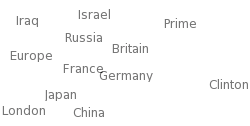
\includegraphics[width=0.32\textwidth]{figures/03_theory/03_wordEmbeddings1}
    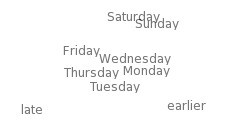
\includegraphics[width=0.32\textwidth]{figures/03_theory/03_wordEmbeddings2}
    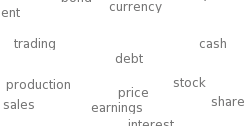
\includegraphics[width=0.32\textwidth]{figures/03_theory/03_wordEmbeddings3}
    \caption[\textbf{Three regions of a word embedding visualized by t-SNE.} Source: Turian et al.~\cite{Turian2010} -- Source for full image \url{http://metaoptimize.s3.amazonaws.com/cw-embeddings-ACL2010/embeddings-mostcommon.EMBEDDING_SIZE=50.png}]{Three regions of a word embedding visualized by t-SNE. The left region contains names of countries, the middle region consists of days and the right regions is made up of financial terms. Source: Turian et al.~\cite{Turian2010}\protect\footnotemark}
    \label{fig:03_WordEmbeddings}
\end{figure}
\footnotetext{Full source for image \url{http://metaoptimize.s3.amazonaws.com/cw-embeddings-ACL2010/embeddings-mostcommon.EMBEDDING_SIZE=50.png}}

For many \gls{nlp} tasks, word representations have become indispensable and one of the factors of success for many systems~\cite{Luong2013}. The next sections showcase a few of the most popular embedding techniques.

\subsection{Word2Vec}
\label{sec:03_word2vec}

Word2Vec by Mikolov et al. is a well-known method which learns to produce word embeddings unsupervised from raw text~\cite{Mikolov2013}. The authors propose two approaches to learn an embedding. Both are very similar and rely on shallow neural networks to generate useful embeddings. Moreover, these methods are computationally much more efficient than previous architectures without sacrificing performance. This efficiency allows word2vec to be applied on much bigger corpora with billions of words which was not possible before~\cite{Mikolov2013c}.


\subsubsection*{Skip-gram Model}

The training objective for the skip-gram model is to predict the neighborhood context of a given word. For example, given the word $w_t$ and a window size of 2 the objective is to predict the two words before $w_t$ {($w_{t-2}, w_{t-1}$)} as well as the two words after $w_t$ {($w_{t+1}, w_{t+2}$)}. The objective can be formalized as maximizing the average log probability~\cite{Mikolov2013e}:

\begin{equation}
\frac{1}{T} \sum_{t=1}^T \quad \sum_{-c\leq j \leq c, j \neq 0} log p(w_{t+j} | w_t)
\end{equation}

$T$ is the number of words in the corpus, $c$ is the context window size and $p(w_{t+j} | w_t)$ is the softmax function. Simply put, skip-gram predicts a context given a source word.

\subsubsection*{\acrfull{cbow}}

\gls{cbow} is very similar to the skip-gram model. However, instead of predicting context words for a source word, \gls{cbow} predicts the next word $w_{t}$ in a sequence, given the previous words $w_{t-j}$~\cite{Mikolov2013c}. In some instances, the surrounding words are taken as the context instead of just the previous words. In other words, the objective of \gls{cbow} is to predict a word given its context.
\medskip

Skip-gram works better for smaller datasets than \gls{cbow} since it is possible to generate more training pairs from a sequence. In addition, it is also able to represent rare words better than \gls{cbow}. However, \gls{cbow} is faster to train than skip-gram and yields slightly better accuracy for more common words.

\subsection{\acrfull{glove}}

There are two methods to create word vectors: word co-occurrence counting {(Section~\ref{sec:03_vectorSpace})} and the window based skip-gram / \gls{cbow} methods {(Section~\ref{sec:03_word2vec})}. Co-occurrence is relatively fast and efficient to collect and train unless the vocabulary is huge. A co-occurrence matrix also captures a lot of global statistical information whereas local window based models only capture the statistics for the window. However, most of the information a co-occurrence matrix provides is about the word similarity and not necessarily about the semantics. In addition, frequent words like "the" or "a" co-occur with a lot of other words. Therefore, they have huge co-occurrence counts with many words without providing any useful information~\cite{Pennington2014a}.

Local window based models like word2vec have the disadvantage that training is not as efficient and these models do not capture a lot of statistical information~\cite{Pennington2014a}. 
\medskip

\gls{glove} which was introduced by Pennington et al. tries to combine the advantages of both model families~\cite{Pennington2014a}. \gls{glove} captures the global corpus statistics directly by creating a co-occurrence matrix $X$ where the entry $X_{ij}$ denotes how often the word $j$ occurs together with $i$. The probability that $i$ appears in the context of $j$ is 

\begin{equation}
    P_{ij}=P(j|i)=\frac{X_{ij}}{X_i}=\frac{X_{ij}}{\sum_k X_{ik}}\quad.
\end{equation}

To put it simply, $P_{ij}$ is just the number of times $i$ and $j$ appeared together divided by the sum of all words that $i$ appeared with~\cite{Pennington2014a}.

Pennington et al. demonstrate that the ratio of probabilities $P_{ik} / P_{jk}$  encodes a lot of the meaning that is lost in traditional co-occurrence based methods~\cite{Pennington2014a}.
\medskip

The authors use $F$ to describe this ratio as

\begin{equation}
    F(w_i, w_j, \widetilde{w}_k) \approx \frac{P_{ik}}{P_{jk}}
\end{equation}

$w$ are just word vectors of $i$, $j$ and {($\widetilde{w}_k$)} is a context vector. In the end the goal is to get a good candidate for $F$ that fulfills all our requirements. To get word vector arithmetic the authors propose to add the vector differences {($w_i - w_j$)} and linear relations {(dot-product)}. So $F$ becomes

\begin{equation}
    F((w_i - w_j)^T \cdot \widetilde{w}_k) \approx \frac{P_{ik}}{P_{jk}} \quad .
\end{equation}

By replacing the probability ratio with logarithms, we arrive at

\begin{equation}
    w_i^T \cdot \widetilde{w}_k = log(P_{ik}) = log(X_{ik}) - log(X_i) \quad .
\end{equation}

The weighted least squares objective function is then finally

\begin{equation}
    J = \sum_{i,j=1}^V f(X_{ij}) (w_i^T \cdot \widetilde{w}_k + b_i+\widetilde{b}_j - log(X_{ij})^2)
\end{equation}

where $V$ is the vocabulary size and $b$ and $\widetilde{b}$ are bias terms which are added.
\medskip

The last problem is solved by a weighting function $f(X_{ij})$. Co-occurrences which are infrequent contain much noise. Therefore, it is important to reduce the influence of noisy words and prevent common words like "the" from dominating the model. Therefore, they weight each word to make sure that words are not over or underrepresented.

\subsection{FastText}

FastText is an embedding technique which focuses on efficiency but is still on par with other word embedding techniques~\cite{Joulin2016}.
\medskip

FastText is based on Word2Vec. However, whereas word2vec treats each word as an atomic entity, FastText splits words into several character n-grams. The word "where" consists of the following 5 $n$-grams for $n=3$~\cite{Bojanowski2017}: 

\begin{center}
    "\verb|<wh|", "\verb|whe|", "\verb|her|", "\verb|ere|", "\verb|re>|"
\end{center}

The special characters "<" and ">" are boundary symbols to differentiate prefixes and suffixes from the beginning and ending of words~\cite{Bojanowski2017}.
\medskip

This notion is very powerful since it provides several advantages over previous models. For one, out of vocabulary words are better recognized since their $n$-grams are still known. Unknown words can, therefore, be partly constructed by known $n$-grams.~\cite{Bojanowski2017}. 
\medskip

Some languages like German which heavily rely on compound words also profit from this technique since those words can also be constructed using known $n$-grams~\cite{Bojanowski2017}.
\medskip

Lastly, FastText represents rare words a lot better than word2vec. Even if a word is scarce and only occurs in a sentence a few times in total, there is a high chance that the model consists of $n$-grams which appear in other, more frequent words~\cite{Bojanowski2017}.

\section{Google Transformer Architecture}
\label{sec:03_transformer}
The Google transformer architecture is a novel neural network architecture for automated machine translation tasks by Vaswani et al.~\cite{Vaswani2017d}. Instead of relying on \gls{rnn} based architectures with recurrence, the transformer uses an attention mechanism to achieve \gls{sota} results on machine translation tasks. Like most of the sequence-to-sequence models the transformer also uses the encoder-decoder pattern to translate a sentence from the source to the target language. This work mostly focuses on the encoder part of the model since this is the part, we use to perform \gls{absa} classification.
\medskip

The issue when training many \gls{rnn}-based architectures is the problem of long-range dependencies. These dependencies may lead to either vanishing or exploding gradient~\cite{Hochreiter2009}. The dilemma is, that language translation features a lot of long dependencies. For some translations like "I like planes" to "Ich mag Flugzeuge" each token exactly matches the position of the translation. However, in many cases the positioning of words is different. Take the sentence "I think I \underline{saw} you at the airport \emph{yesterday}." This sentence translates to "Ich glaube, dass ich dich \emph{gestern} im Flughafen \underline{gesehen habe}".

When translating this sentence from English to German, a recurrent architecture has to keep the dependency of "\underline{saw}" all the way until the end of the German sentence when it has to output the tokens "\underline{gesehen habe}".
\medskip

Besides the issue with long-term dependencies, \gls{rnn} architectures are also almost impossible to parallelize which is especially crucial for long sequences~\cite{Vaswani2017d}.
\medskip

The transformer model tries to fix both problems. It is the first transduction model to completely give up on recurrence or convolutions to compute sequence representations~\cite{Vaswani2017d}. 

Instead, it relies on attention and specifically multi-head attention. Attention allows a model to focus on relevant information and the idea of multi-head attentions enables parallelization as well as attention heads which focus on their attention on different aspects~\cite{Vaswani2017d}.

\subsection{Encoder-Decoder Architecture}

\begin{figure}[htp]
    \centering
    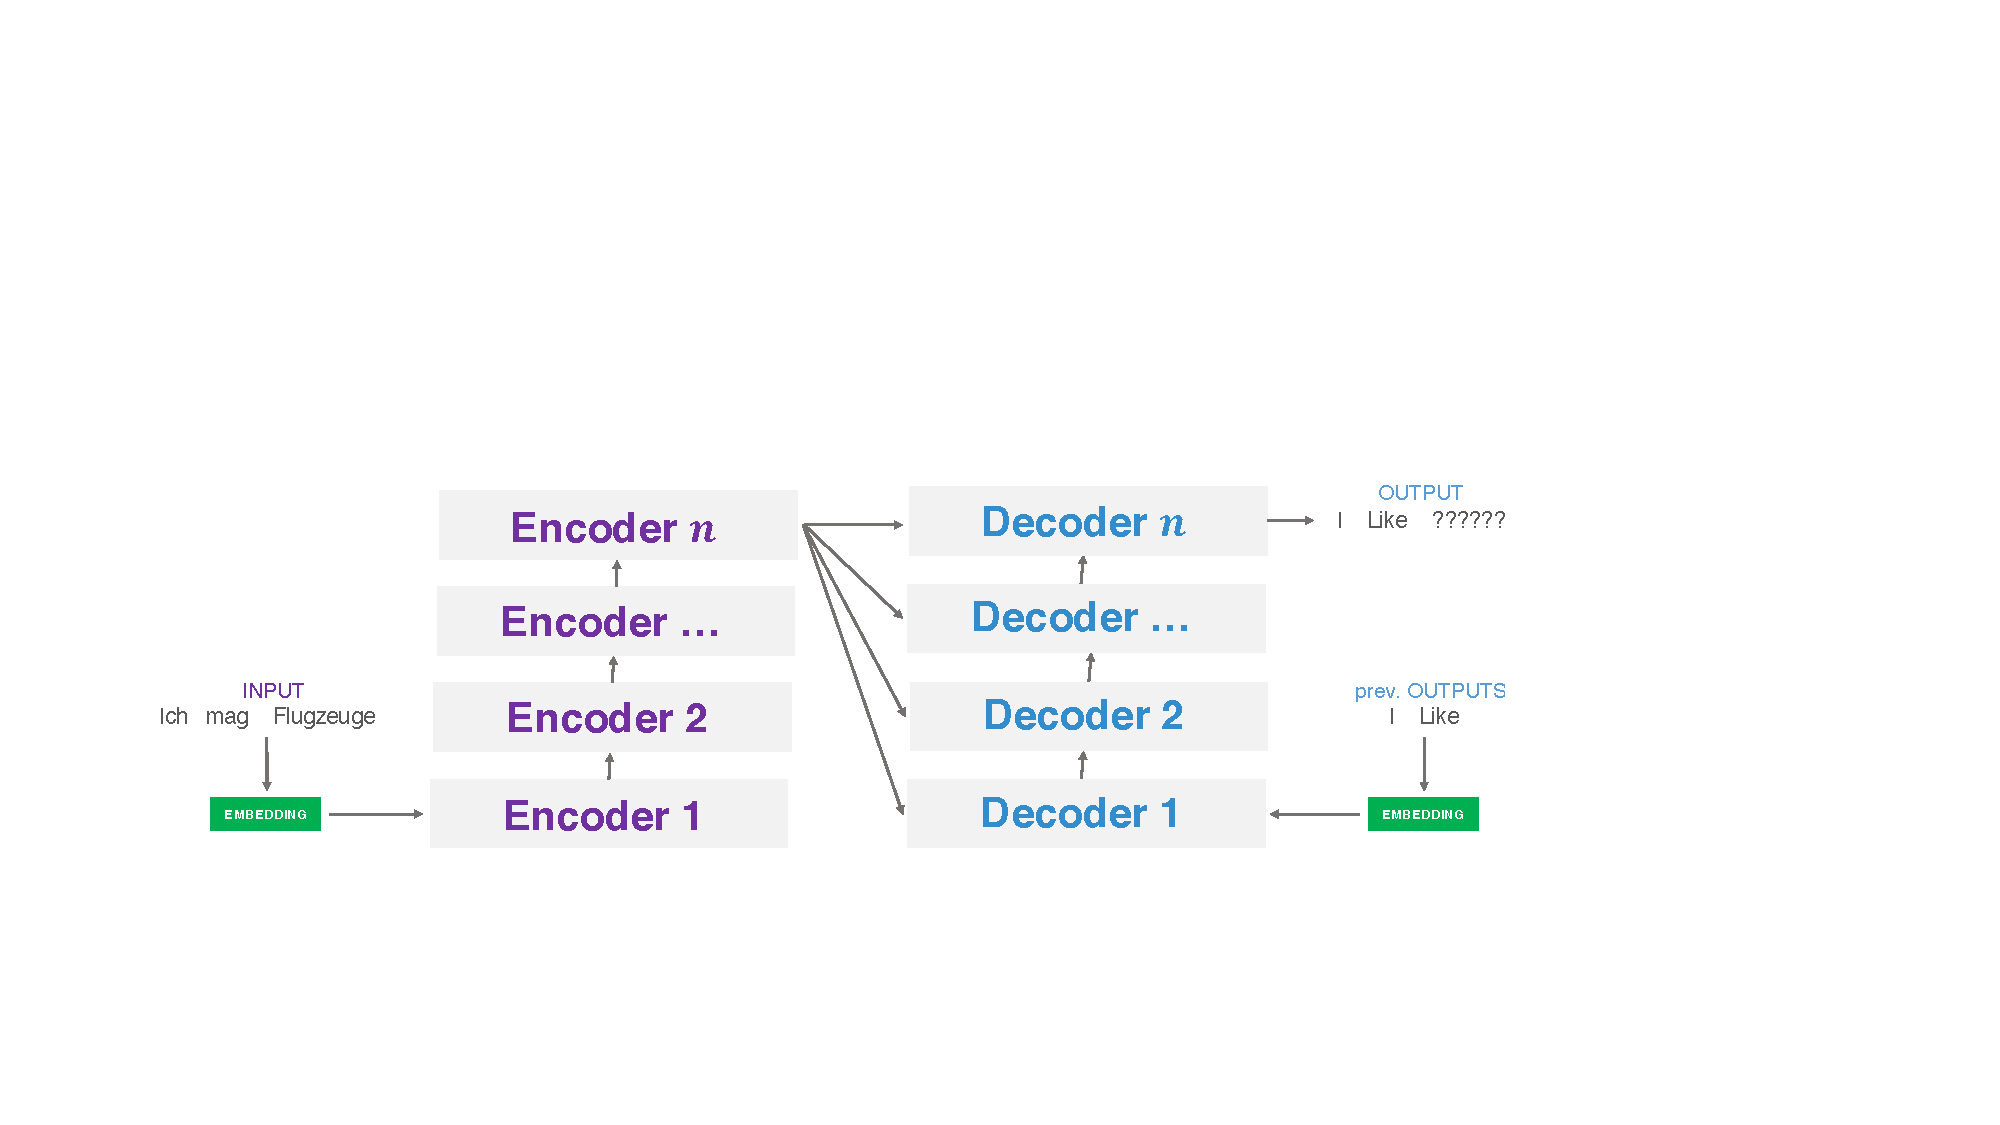
\includegraphics[width=\textwidth]{figures/03_theory/03_transformer_Architecture_HighLevel}
    \caption{\textbf{High-level overview of the transformer Encoder-Decoder architecture}, translating the sentence "I mag Flugzeuge" from German to English. The model is at the step where it translates the last word "Flugzeug" to plane.}
    \label{fig:03_transformer_HighlevelOverview}
\end{figure}

Figure~\ref{fig:03_transformer_HighlevelOverview} depicts a high-level architectural overview of the transformer. As already mentioned the transformer resembles an encoder-decoder architecture. Yet, in contrast to traditional encoder-decoders, the transformer consists of $n$ encoder- and $n$ decoder blocks~\cite{Vaswani2017d}. 
\medskip

The first encoder block gets the whole input sequence encoded as word vectors. This sequence is then propagated until it reaches the top encoder. From there, the encoder output is passed to all decoder blocks. Furthermore, the decoder blocks also receive the output of the decoder blocks below them. In addition, the first decoder block {(in figure~\ref{fig:03_transformer_HighlevelOverview} this block is named "Decoder 1")} receives the sequence of tokens the transformer already predicted~\cite{Vaswani2017d}. 
\medskip

Following the example in figure~\ref{fig:03_transformer_HighlevelOverview} the translation would start by passing the sentence "\textit{Ich mag Flugzeuge}" through all encoder blocks until it reaches the top block. All 1 to $n$ decoder blocks receive the encoded sentence. The encoded sentence then flows up from Decoder 1 to the top where Decoder $n$ outputs the first token "\textit{I}".

Decoder 1 now gets two inputs: 

\begin{enumerate}
    \item the encoded source sentence from the encoders it previously also received
    \item the previously predicted output from the decoders which is the token "\textit{I}".
\end{enumerate}

Decoder 2 to $n$ now get the encoded input {(as before)} as well as the output of the decoders below. The top encoder then outputs "\textit{like}" as the next token in the sequence. 

Figure~\ref{fig:03_transformer_HighlevelOverview} displays the next step that would follow this one where "\textit{I like}" is already predicted and only the last token is missing.
\bigskip

To gain a complete understanding of the information flow on the encoder and decoder side, Figure~\ref{fig:03_transformer_overview} shows a detailed overview of one encoder and one decoder block.

\begin{figure}[t]
    \centering
    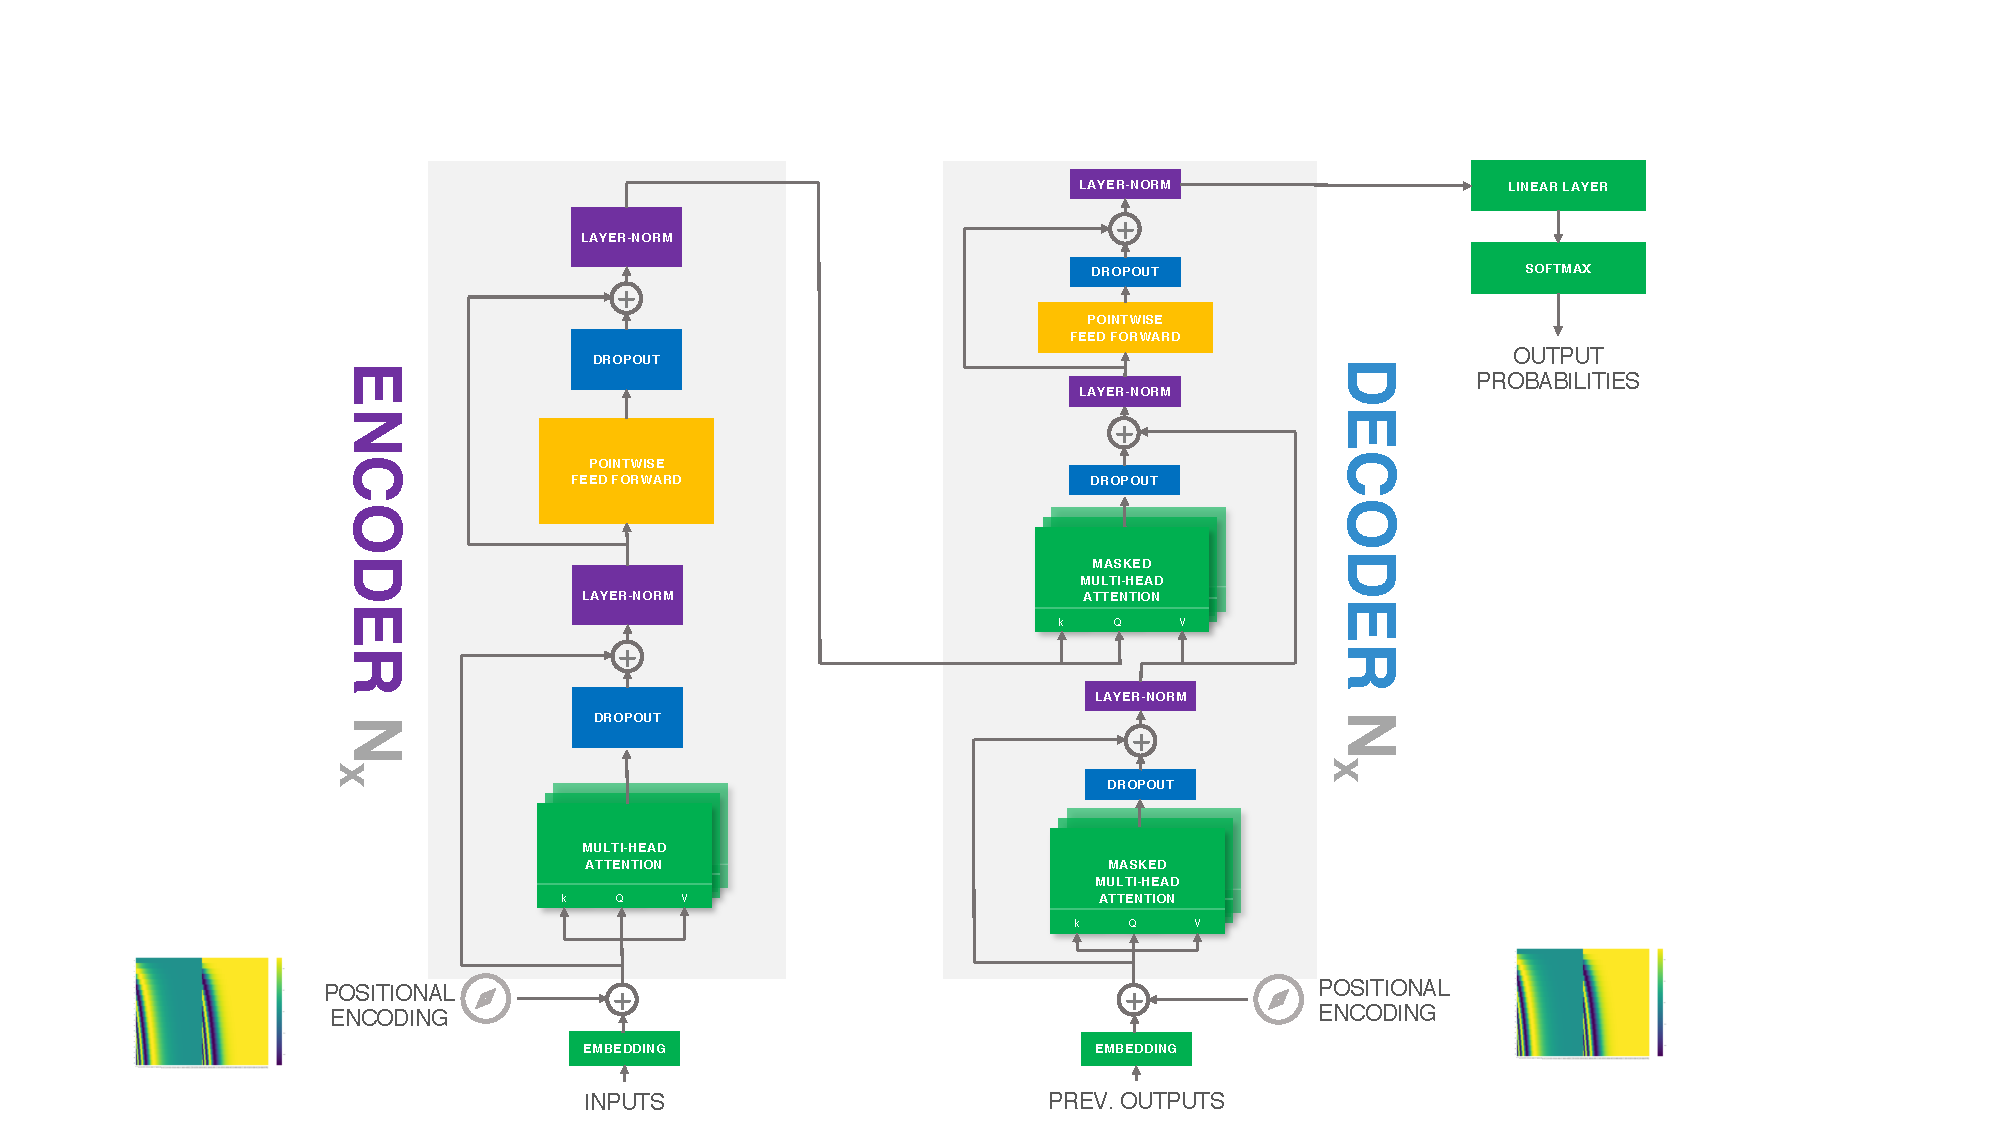
\includegraphics[width=\textwidth]{figures/03_theory/03_transformerArchitectureOverview}
    \caption{\textbf{Overview of the whole Transformer architecture}. This figure shows both the encoder and the decoder stacks as well the information flow between the encoder and the decoder.}
    \label{fig:03_transformer_overview}
\end{figure}

\subsection{Attention Mechanism}

The transformer uses attention to focus on the essential and relevant information in a sequence. The question of what is regarded as important is learned~\cite{Vaswani2017d}.

The specific attention mechanism, the transformer uses is called "Scaled Dot-Product Attention" {(Figure~\ref{fig:03_transformer_scaledDotProduct} left)}. The input for the attention function are three matrices called "Queries" $Q'$, "Keys" $K'$ and "Values" $V'$.

In case of the encoder stack, these matrices are the input word embeddings. We multiply the embeddings with $W^Q$, $W^K$ and $W^V$. These projection matrices are learned and project our input to a lower dimension $d_q$, $d_k$ and $d_v$ so that we get $Q', K', V'$~\cite{Vaswani2017d}.
\bigskip

We then take the dot-product of $Q'$ and $K'$ and scale the result by dividing by the square root of $d_k$ where $d_k$ is the dimension of $Q'$ and $K'$. Next, we can finally apply the attention. From the softmax, we get a vector of probabilities which are the attention values. When we apply the dot product on those attentions and the values, we scale the values with the attentions~\cite{Vaswani2017d}. Refer to Figure~\ref{fig:03_transformer_scaledDotProduct} for a visualization of this process.
\medskip

Words which are deemed relevant by the attention mechanism are multiplied with values near 1 while unimportant words are multiplied with small values and therefore become unimportant for the next layers~\cite{Vaswani2017d}.
\medskip

One aspect which was not yet mentioned is the "mask"-step. After the scaling operation, we need to set some values to 0. We perform this masking because every input sequence needs to have the same length which we achieve by adding <pad> tokens to sentences which are not long enough. Those tokens carry no information so we can safely discard them in this step~\cite{Vaswani2017d}. 

In the decoder part, we need to mask specific parts of the sentence which the transformer has not predicted yet. This operation is done to prevent the model from cheating by just replaying the input sequence~\cite{Vaswani2017d}.
\medskip

Vaswani et al. constructed the transformer to use multiple "attention-heads" where each "head" performs its own dot-product attention {(Figure~\ref{fig:03_transformer_scaledDotProduct} right)}. 

To get different values for the attention, each head $i$ has its own set of $W_i^Q$, $W_i^K$ and $W_i^V$ matrices. The main idea behind the concept of multi-head dot-product attention is that each head specializes on some aspect. One head might pay attention to entities while another head looks out for actions~\cite{Vaswani2017d}. This being said, in practice, it is not as clear what each head focuses on, and the distinction is fuzzier.

The following equation summarizes the process which is described above and visualized in Figure~\ref{fig:03_transformer_scaledDotProduct}:
\begin{align}
    \text{Attention}(Q', K', V') & = \text{softmax}(\frac{Q' \cdot K'^T}{\sqrt{d_k}}) \cdot V' \\
    \text{AttentionHead}_i(Q, K, V) & = \text{Attention}(QW_i^Q, KW_i^K, VW_i^V)
\end{align}

\begin{figure}[htp]
    \centering
    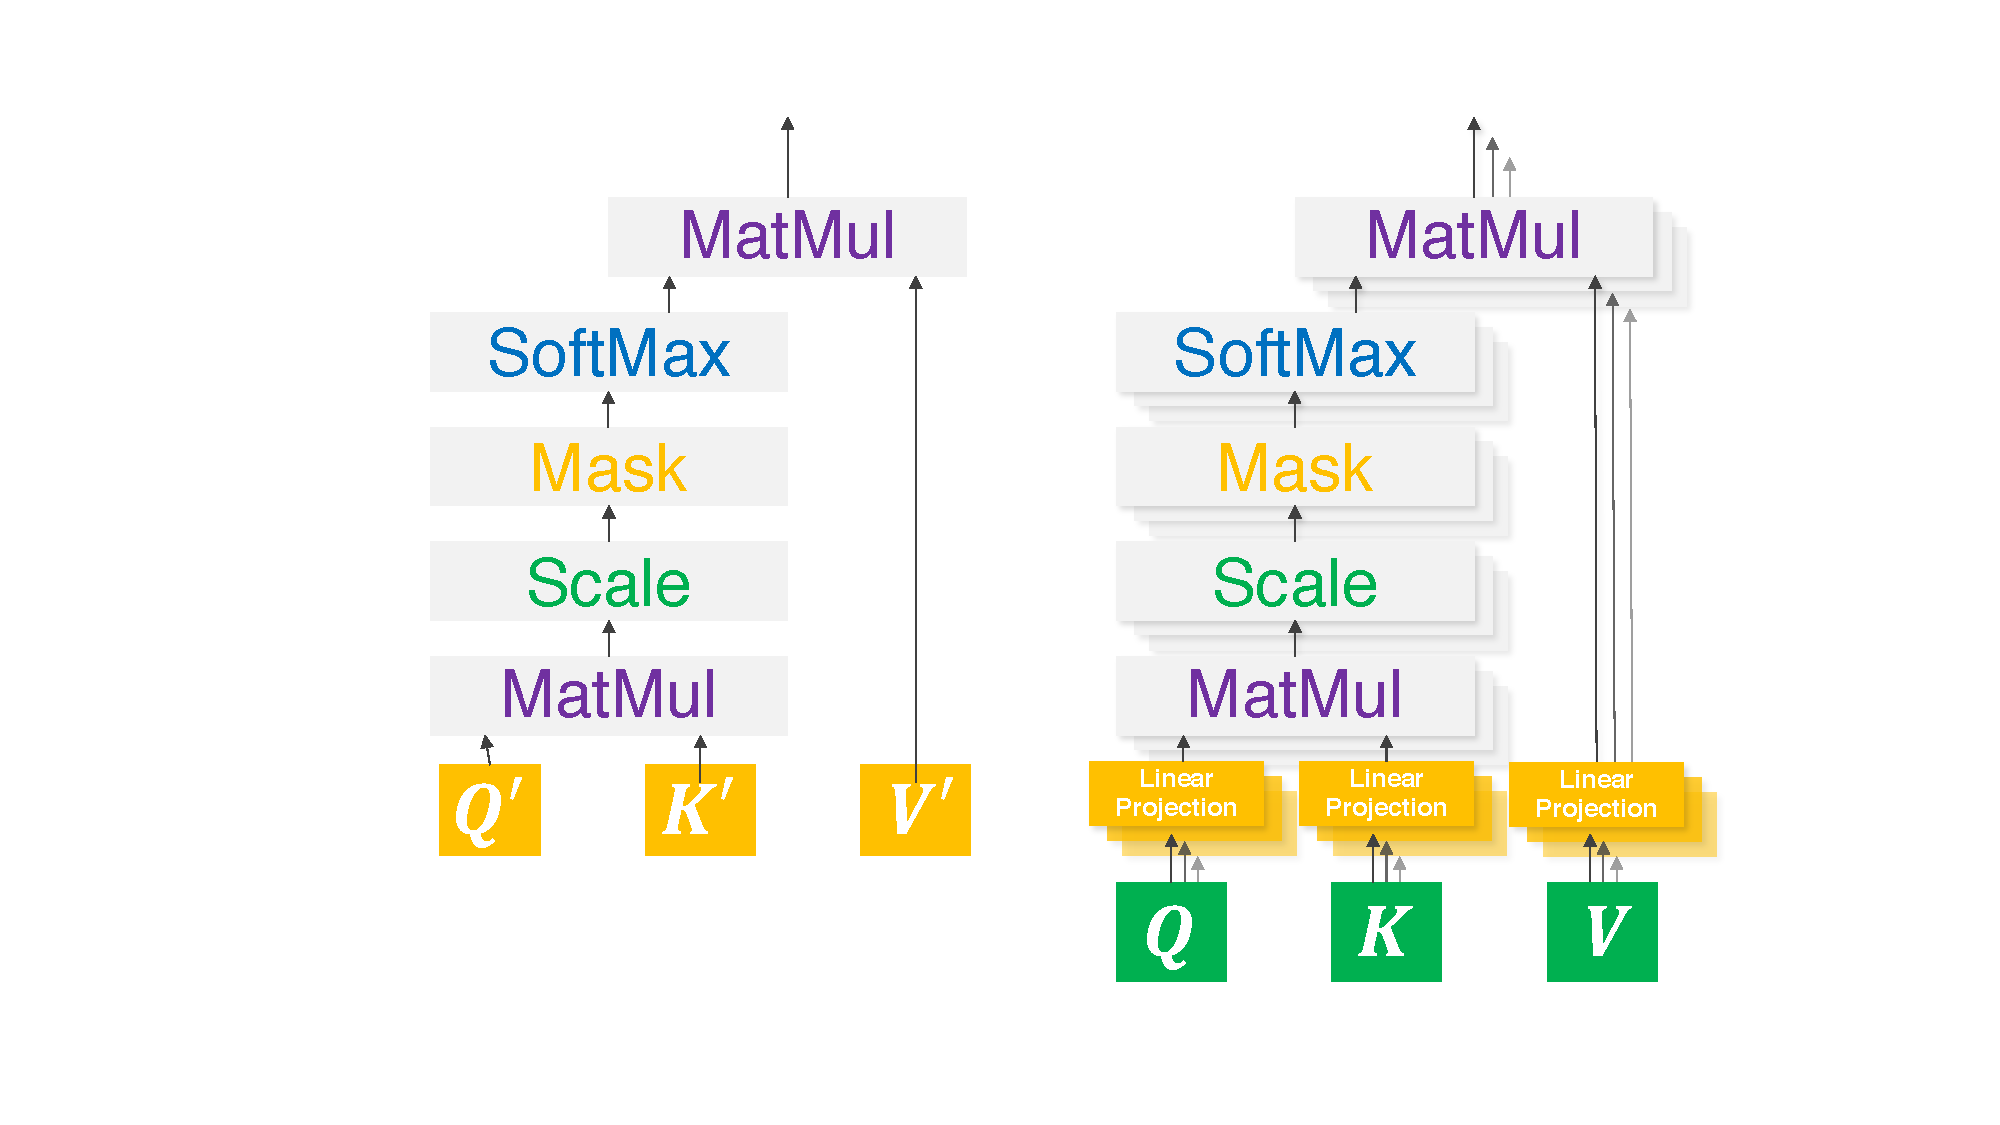
\includegraphics[width=0.7\textwidth]{figures/03_theory/03_transformer_ScaledDot}
    \caption{\textbf{Attention and Multi-head Attention}. left: single scaled dot-product attention mechanism. right: multiple scaled dot-product attention heads stacked together. Each head receives its representation of $Q$, $K$ and $V$ by using projection layers.}
    \label{fig:03_transformer_scaledDotProduct}
\end{figure}

\subsection{Positional Encoding}

The transformer always gets the complete sequence of words as the input. However, since the transformer has no recurrence, it has no memory. As a consequence, it does not know which word is at which position. However, the order of words is essential to understand sentences~\cite{Vaswani2017d}. 
\medskip

A "positional encoding" solves this issue. For the positional encoding, the authors use a combination of sine and cosine functions. They also experimented with a learned encoding, but this approach did not yield any significant performance improvements~\cite{Vaswani2017d}.

This encoding is added to the word embeddings at the bottom of the encoders and decoders. It has the same dimension as the embedding so it can be added element-wise~\cite{Vaswani2017d}.


\subsection{Point-wise Layer}

After the transformer passes the input through the attention heads, it uses a pair of fully connected layers with nonlinearities~\cite{Vaswani2017d}. 

The first linear layer scales the input to the inner layer dimensionality of 2048 and the second layer scales the input back to the previous model size of 512~\cite{Vaswani2017d}.

\subsection{\gls{adam} Optimizer}

Vaswani et al. propose to use the \acrfull{adam} optimizer~\cite{Kingma2014}. \gls{adam} is an extension to the popular \gls{sgd} optimizer. However, instead of having a fixed learning rate like \gls{sgd}, Adam computes a learning rate for each trainable network parameter. Those learning rates are directly obtained by the decaying mean and uncentered variance of the past gradients~\cite{Kingma2014}.
\medskip

This is different from AdaGrad~\cite{Duchi2011} and RMSProp~\cite{Hinton} which also maintain a learning rate for each parameter. However, RMSProp only uses the mean of past gradients and AdaGrad updates parameters based on how frequent the specific parameter is used as a feature.

\section{Multi-Task Learning}

Rich Caruana first introduced \acrfull{mtl} in 1993. Conventional machine learning approaches break a problem down in smaller tasks and solve one task at a time (e.g., word-by-word \gls{pos}-tagging~\cite{Toutanova2007}, word-by-word \gls{ner}~\cite{Sang2003} or handwritten image classification~\cite{LeCun;1990}). In each of these tasks, a classification algorithm solves exactly one task (Assigning a 'part-of-speech' or entity type to a word, or the classification of handwritten digits). Caruana shows that combining multiple related tasks improves model performance~\cite{Caruana1993, Caruana1997a}. 

In \gls{mtl}, multiple related tasks are learned in parallel and share a common representation. Generally speaking, every machine learning model which optimizes multiple objectives for a single sample can be considered as Multitask Learning. This definition includes multi-label classification where one sample can have multiple labels as well as instances where different sample distributions or datasets are used for different tasks.

\gls{mtl} is similar to how humans learn. Generally, humans learn new tasks by applying knowledge from previous experiences and activities. For instance, it is easier to learn ice skating when someone previously learned inline skating. This is because all the essential underlying aspects of the tasks are very similar.

When tasks are related this also holds for machine learning. When learning these tasks in parallel model performance is improved compared to learning them individually since the additional knowledge that a related task carries can be used to improve on the original task~\cite{Caruana1997a}. 

There are four important aspects one can use to determine if \gls{mtl} can bring performance boosts for a specific objective:
\begin{enumerate}
    \item \textbf{Multi-Label Task}: A Multi-Label classification task where one sample has more than one label is almost always inherently solved using \gls{mtl} if one model predicts multiple labels. Various authors show that adding tasks always improves performance compared to a separate model for each task as an alternative~\cite{Ramsundar2015}.
    \item \textbf{Shared low-level features}: \gls{mtl} only makes sense if the tasks share low-level features. For instance, image classification and \gls{nlp} do not share common features. In this case, the model would not benefit from \gls{mtl} because one task can not help to improve the other task. Therefore, it is important to choose tasks that are related to each other~\cite{Zhang2017a}. In most cases, \gls{mtl} works with \gls{nlp} tasks because they usually share at least some kind of sentence or word embedding as a common layer.
    \item \textbf{Task Data Amount}: Several authors have suggested that it is important for the success of \gls{mtl} training that the amount of data for the tasks is similar. Otherwise, the model mainly optimizes for the task with most training samples.
    \item \textbf{Model Size}: Finally, the multi-task model needs to have enough parameters to support all tasks~\cite{Caruana1997a}. 
    \end{enumerate}


\subsection{Differentiation against Transfer Learning}

Training samples from one task can help improve the other task and vice versa. This aspect is important for the differentiation against transfer learning~\cite{Pratt1993}. In \gls{mtl} each task is equally important. In transfer learning the source task is only used to improve the target task. So the target task is more important than the source task~\cite{Zhang2017a}. In addition, Transfer Learning uses a linear training timeline. First, the source task is learned and then after learning is completed this knowledge is applied to boost the learning process of the target task. When performing \gls{mtl}, in contrast, the model is learning both tasks jointly together instead of one after the other.


\subsection{Improvements through Generalization}
\label{sec:03_mtlAdvantages}

There are several reasons why the \gls{mtl} paradigm performs so well. For instance, the generalization error is lower on shared tasks~\cite{Caruana1993}. \gls{mtl} acts as a regularization method and encourages the model to accept the hypothesis that explains more than one task at the same time~\cite{Ruder2017}. The model is forced to develop a representation that fits the data distributions for all tasks. In the end, this creates a model that generalizes better because it must attend to different objectives.

\subsection{Improvements through Data Augmentation}

Secondly, Multi-Task Learning increases the number of available data points for training. All tasks share a common representation. While training one task, all other tasks are also implicitly trained through the joint representation~\cite{Caruana1993}.

\subsubsection*{Statistical Data Amplification}

Each new task also introduces new noise. Traditionally, a model tries to learn by ignoring the noise from its data. However, if the model does not have enough training samples it will overfit because it focuses too much on the noise to explain the data. By introducing additional tasks, new data and therefore new noise is introduced which the model has to try and ignore~\cite{Ruder2017}. This aspect is called \textit{Statistical Data Amplification}\cite{Caruana1995a}.

\subsubsection*{Blocking Data Amplification}

\textit{Blocking Data Amplification} occurs when there is little or no noise. Consider the simple example from Caruana~\cite{Caruana1995a}.

There are two tasks $T_1$ and $T_2$ and common features $F$. The first task $T_1$ is $T_1 = A \land F $ and the second task $T_2$ is $T_2 = \neg A \land F$. 

For $A=0$ only $T_1$ uses feature $F$ and $T_2$ does not. For $A=1$ it is the other way around. By training on both tasks, $F$ is used no matter what value $A$ takes. 
\medskip

Rei makes use of these aspects and proposed a sequence labeling framework which uses a secondary, unsupervised word prediction task to augment other tasks such as \gls{ner} or chunking. Rei demonstrates that by including the auxiliary word prediction task, the source task performance is improved for all sequence labeling benchmarks the author tried~\cite{Rei2017}.
\medskip

Similarly, Plank et al. show that learning to predict word-frequencies along with \gls{pos}-tagging also improves the total model performance~\cite{Plank}. They argue that predicting word frequencies helps to learn the differentiation between rare and common words.


\subsection{Architecture}
The most common architecture for multitask learning is shown in figure~\ref{fig:03_mtl_architecture}. It is called hard parameter sharing and consists of at least one layer which is shared among all tasks. In addition, each task has at least one separate layer. This approach is also the one we used for our model which we describe in Chapter~\ref{ch:method}. 

The easiest way to compute the loss for a hard parameter sharing \gls{mtl} architecture is to take the sum of all losses for the individual tasks which is shown in equation \ref{eq:04_multiheadLoss}.

% TODO: redo figure 
\begin{figure}[ht]
    \centering
    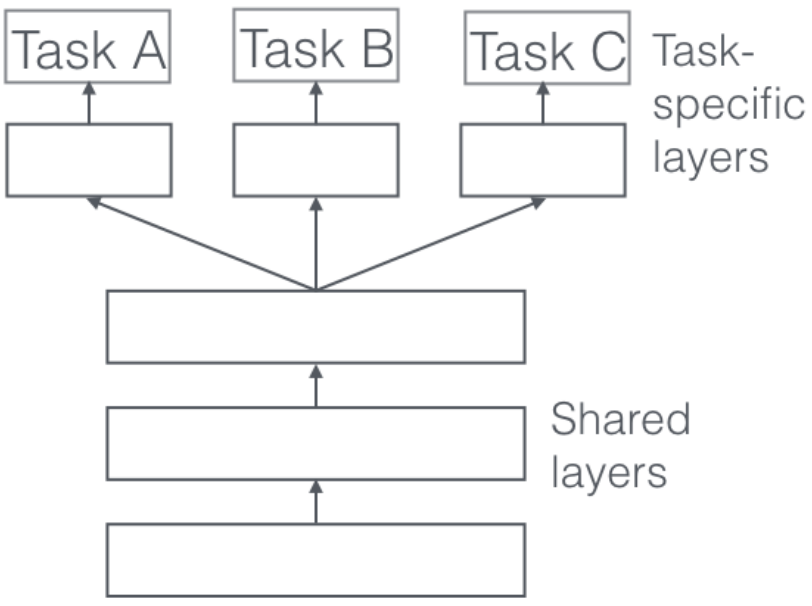
\includegraphics[scale=0.5]{figures/03_theory/03_mtl_architecture}
    \caption{\textbf{Hard parameter sharing}. The first three layers are shared among tasks A, B and C. Each task also has one or more layers. Source: Ruder 2017~\cite{Ruder2017}}
    \label{fig:03_mtl_architecture}
\end{figure}

\section{Transfer Learning}
\label{sec:TransferLearning}

In 1991, Pratt et al. suggested to transfer information encoded in a neural networks by reusing the network weights in a new network~\cite{Pratt1991}. They show that even accounting for the training time of the source network they achieve significant speedups when training a target network compared to random weight initialization.
\medskip

Yosinski et al. provide a more modern definition: First, a base network is trained on a source dataset. Then, the learned features {(the knowledge)} of the base network is transferred to a second target network which is then trained on the target dataset and the target task~\cite{Yosinski2014}. 

This process works well if the base and target dataset and tasks are similar.
\medskip

Goodfellow et al. give a more general definition. They define \gls{tl} as the transfer of previously learned knowledge from one or multiple sources to a target domain with fewer examples~\cite{Goodfellow2016}.

Figure~\ref{fig:03_transferLearning} communicates those definitions and compares traditional machine learning to transfer learning.
% TODO: redo figure 
\begin{figure}[ht]
    \centering
    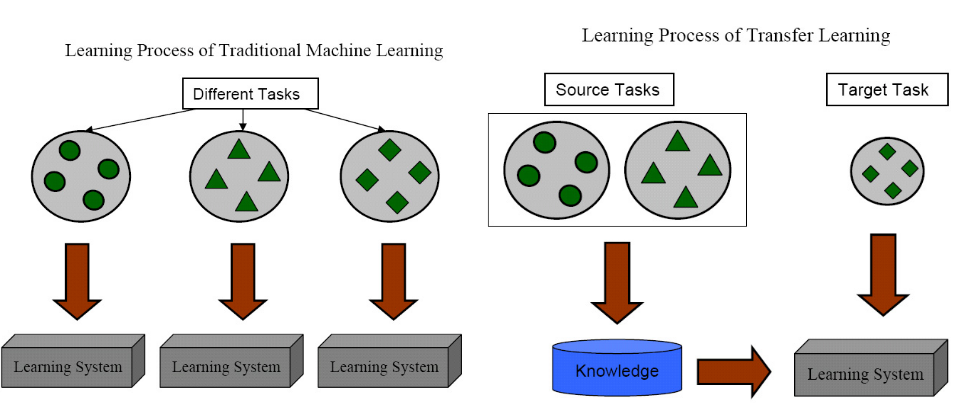
\includegraphics[scale=0.55]{figures/03_theory/03_transferLearning}
    \caption{\textbf{Visualization of Transfer Learning and comparison against traditional learning.}This figure shows the difference in traditional machine learning were each model uses its own dataset and task. In contrast, in transfer learning a model is first trained on source tasks and part of the features are transformed to the target model to facilitate training. Source: Pan and Yang~\cite{Pan2010}}
    \label{fig:03_transferLearning}
\end{figure}

\subsection*{Motivation}

In practice, it is costly to collect or recollect training data for every new domain. Transfer learning makes it possible to transfer knowledge from a larger dataset to a smaller dataset which dramatically reduces the labeling effort~\cite{Blitzer2007}. Studies show that it is possible to train large networks on small target datasets without overfitting when the model has been trained on a large dataset before~\cite{Donahue2013, Zeiler2014}. 

Usually, after the base model has been trained on the large dataset, the first $n$ layers of the base model are copied over as the first $n$ layers of the target model. The remaining layers of the target model are then randomly initialized and trained. The weights of the $n$ layers from the base model can either be \textit{frozen} or \textit{finetuned} along the rest of the target model. 

If the target dataset has few samples and the number of parameters in the first $n$ layers is high, finetuning can actually result in overfitting. As a consequence, researchers often chose not to backpropagate the error during target training all the way to the first $n$ layers~\cite{Yosinski2014}.

\subsection*{Pre-Training}
The most common way to employ transfer learning is pre-training. 
Pre-training is often used in image recognition where interestingly, the first few layers generally form into the same feature regardless of the domain or task~\cite{Yosinski2014}. Consequently, researchers can exploit this by taking the first layers from a model which was previously trained on a large dataset like ImageNet~\cite{Russakovsky2015} and use these weights for their tasks which might have fewer examples.
\medskip

This paradigm can also be applied to natural language processing. Understanding what words mean is the fundamental problem every \gls{nlp} model needs to solve. Therefore, it is sensible to use an embedding layer which has been pre-trained on large datasets like "common crawl"~\cite{commonCrawl}. Common crawl contains petabytes of information and produces good general word embeddings. This pre-trained embedding layer can then be used in a model trained on a much smaller dataset.
 
\section{Hyperparameter Optimization}

Generally, there are two sets of parameters in machine learning: learned parameters and hyperparameters. Hyperparameters are used to configure various aspects of the training process. Learned parameters such as neural network weights are optimized during training whereas hyperparameters are usually defined at the beginning and without a few exceptions {(e.g. learning rate)} do not change during training.
\medskip

It has been demonstrated that there are a few hyperparameters which have an enormous impact on the overall model performance but identifying those parameters among a big set of possible candidates is difficult~\cite{Bergstra2012a}. However, it is crucial to set these parameters correctly for achieving an excellent model performance. Cox and Pinto demonstrated that hyperparameters make the difference between a state of the art model and a model which does not perform better than a random classifier~\cite{Cox2011}. Therefore, hyperparameter tuning is critical for model performance.
\medskip

Hyperparameters are either hand tuned through literature reviews or by the researchers understanding and intuition of the underlying architecture and how he expects certain parameters to influence the architecture. Another way is to semi-automatically optimize or fully automatically optimize the search for good hyperparameters.
\bigskip

This section presents three approaches to optimize the hyperparameter space. The first two are naive, semi-automatic approaches where a set of possible parameters is tested and the success is recorded. The researcher then selects the most promising results. The third example, Hyperopt, is an algorithm which treats the hyperparameter search as an optimization problem. It tries to indentify critical parameters and tries to find their optimum value for the given model and task~\cite{Bergstra2013}.


\subsection{Grid Search}

Grid search is a straightforward method to search for optimal hyperparameters. When performing a grid search for a parameter, a new value is sampled from a predefined parameter subset at a fixed interval. Each trial with the new parameter value is then evaluated on the model. For multiple parameters each distinct parameter value is tested against all other parameter values, therefore creating a \textit{grid} of parameter values to test.

This approach is very easy to implement and is trivial to parallelize.

\subsection{Random Search}

\begin{figure}[htb]
    \centering
    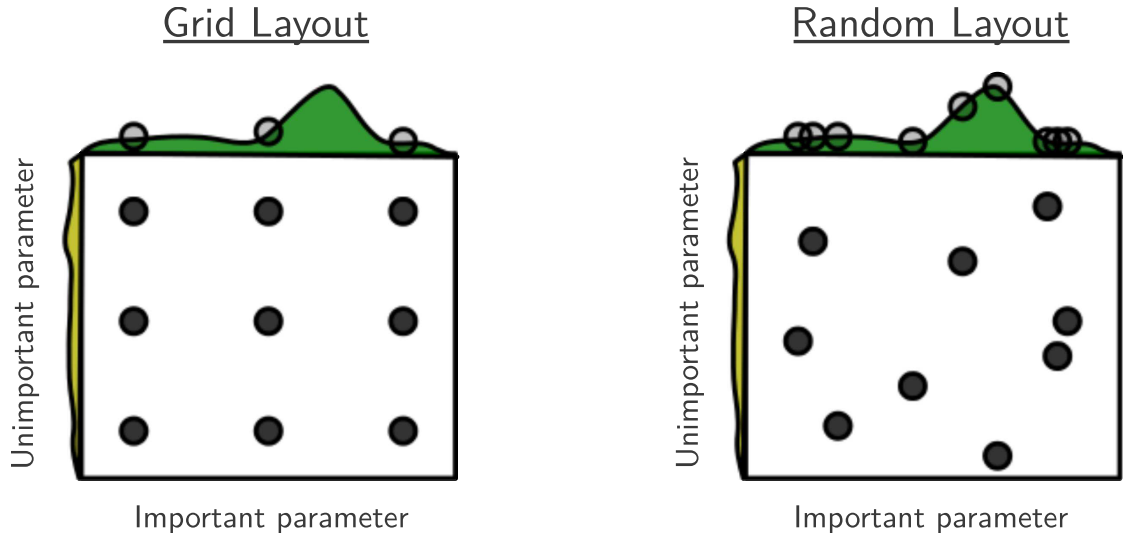
\includegraphics[scale=0.35]{figures/03_theory/03_randomSearch}
    \caption{\textbf{Comparison of Random- and Grid Search.} This figure from Bergstra and Bengio demonstrates the advantage of random searches over grid searches in a two-dimensional space. Nine trials are performed to optimize a function $f(x, y) = g(x) + h(y) \approx g(x)$. $g(x)$ shown in green has a bigger impact compared to $h(y)$ shown in yellow on the left. Each gray circle represents a trial. Because of the two-dimensional space, grid search can only test $g(x)$ in three places. The Random search tries a different $x$ in every trial and is therefore able to find a value close to the optimum. Source: Bergstra and Bengio~\cite{Bergstra2012a}}
    \label{fig:03_randomSearch}
\end{figure}

Surprisingly, Bergstra and Bengio show that randomly choosing hyperparameters is more efficient than performing a grid search~\cite{Bergstra2012a} for high dimensional search spaces. Instead of defining values in a grid, they randomly sample from the grid space.

The problem with grid search is that by increasing the number of dimensions, the number of trials has to increase exponentially to provide the same number of distinct trials for a single parameter~\cite{Bergstra2012a}. When performing a grid search on a one-dimensional parameter space, three runs on the model have to be performed to test three distinct values of the parameter. Optimizing two parameters {(shown in figure~\ref{fig:03_randomSearch})} increases the number of runs to $3^2$ and optimizing $n$ parameters $m$ times will lead to $m^n$ runs. 

Grid search is set up on the assumption that each parameter is equally important. However, Bergstra and Bengio have demonstrated that not all parameters are equally significant for the model performance~\cite{Bergstra2012a}. Figure~\ref{fig:03_randomSearch} demonstrates why this is an advantage for random search over grid search. In this specific example, one parameter constitutes more towards model performance than the other. However, grid search can only sample three values for the critical parameter, and it is therefore not able to find the optimum value. According to Bergstra and Bengio, this situation is the norm rather than the exception for grid search~\cite{Bergstra2012a}.

\subsection{Hyperopt}

Hyperopt is an open source\footnote{Official repository \url{https://github.com/hyperopt/hyperopt}} hyperparameter optimization package by Bergstra et al.~\cite{Bergstra2013a}. It treats the hyperparameter search as an optimization problem. Bergstra et al. show that by using \glspl{tpe} and Gaussian processes Hyperopt can find hyperparameters that outperform random searches and traditional manual hyperparameter tuning~\cite{Bergstra2011}.




\subsubsection*{Challenges of Hyperparameter Optimization}

There are certain challenges when treating hyperparameter tuning as an optimization problem. For instance, the parameter search space is often high dimensional and may contain a mix of continuous {(e.g. learning rate)}, discrete {(e.g. hidden layer size)}, boolean {(e.g. preprocessing steps~\cite{Hutter2009})} and even conditional variables~\cite{Bergstra2013}. 

For instance, the choice of an optimizer or even the machine learning algorithm itself can be seen as a hyperparameter. Each choice then has its own set of parameters which are independent of the other choices. For instance, the Adam optimizer uses specific parameters like $\beta_1$ which the \gls{sgd} optimizer does not use. Hyperopt generates a graph from these conditional parameters and then uses a tree-like structure for solving the optimization problem~\cite{Bergstra2011}.
\newline

Another difficulty is the limited "fitness evaluation budget"~\cite{Bergstra2011}. This term means that for each evaluation of a hyperparameter set the model has to be trained. This process potentially takes a long time. Therefore, Hyperopt has to cope with fewer evaluation steps than a standard optimization algorithm.

\subsubsection*{Tree of Parzen Estimators {(TPEs)}}
The Hyperopt package uses \glspl{tpe} to sample good hyperparameters from the hyperparameter search space~\cite{Bergstra2013a}. To model $p(x|y)$ \gls{tpe} replaces, all distributions in the configuration space by Gaussian mixture equivalents:

\begin{itemize}
	\item uniform variables $\rightarrow$ truncated Gaussian mixture
	\item log-uniform variables $\rightarrow$ exponentiated truncated Gaussian mixture
	\item categorical variables $\rightarrow$ re-weighted categorical variables.
\end{itemize}

 The prior for the calculation -- the different observations $\{x^1,..., x^n, ..., x^k\}$ -- is initialized by performing a warmup phase. This phase consists of $n$ random runs where the default value for $n$ is 10.
\medskip

After the warmup phase the \gls{tpe} algorithm defines $p(x|y)$ as

\begin{equation}
p(x|y) =
\begin{cases}

l(x) & \text{if } y < y^* \\
g(x) & \text{if } y \geq y^*

\end{cases}
\end{equation}

where $l(x)$ {(first case)} is a density formed by an observation $\{x^i\}$ where the loss $y$ of $f(x^i)=y$ was less than a threshold $y^*$. This means we pick examples from all previous observations that achieved a "good" loss. This loss value has to be below $y^*$.
\medskip

The threshold value $y^*$ is set to be higher than the loss of the best observation. Consequently, the density $l(x)$ is formed by more than just one observation. 
\smallskip

$g(x)$ is the density we get by using all other remaining observations~\cite{Bergstra2013a}. 
\medskip



$l(x)$ and $g(x)$ model the hyperparameter search space which means that they have to be hierarchical when the search space contains conditional and discrete variables. $l(x)$ and $g(x)$ are then used to optimize the expected improvement and after each iteration the parameter set with the highest expected improvement is chosen for the next iteration which then becomes the next observation $x^{k+1}$~\cite{Bergstra2013a}. 

\section{Performance Measurements}
The following section describes the performance measurement which was used to evaluate the performance of a model.


\subsection{Precession -- Recall -- F1 Score}
The most commonly used measurement for \gls{nlp} tasks is the F1-score. This metric has one advantage over accuracy. Accuracy does not take data imbalance into account. Accuracy is just the number of correctly classified samples divided by the total amount of samples. This means a classifier which predicts the majority class gets a high accuracy.
\medskip

The combination of precision and recall on the other hand, objectively measures the actual relevance and performance of a classifier for a given class. Precision and recall are defined as:

\begin{equation}
Precision = \frac{T_p}{T_p+F_p} \quad Recall = \frac{T_p}{T_p+F_n}.
\end{equation}

\begin{itemize}
    \item True positives $T_P$ is the number of correctly classified samples for a class.
    \item False positives $F_P$ are all samples which the model predicted to be part of the class but are in reality not part of the class. {(Type I Error)}
    \item False negatives $F_N$ are all samples that belong to the class but are labeled as not being part of the class {(Type II Error)}
\end{itemize}

A high recall means that many samples were matched correctly and a high precision denotes a low number of incorrectly classified samples.
\medskip

The F1 score is the harmonic mean between the precision and the recall and is given as

\begin{equation}
    F_1 = 2 * \frac{\text{precision}*\text{recall}}{\text{precision}+\text{recall}}
\label{eq:03_f1}
\end{equation}

The F1 score is scaled from $[0, 1]$ were 0 is a result with no true positive samples. A classifier which achieves a score of 1 classified all samples correctly meaning it has no false positives or false negatives.

\subsubsection*{Micro- and Macro F1 score}
\label{sec:03_macroMicroF1}
There are two popular methods to aggregate the F1 score. Researches can use the micro- or the macro F1 score. Equation~\ref{eq:03_f1} remains the same but the way it is aggregated changes. 
\medskip

The micro F1 score is calculated by taking the sum of all true positives, false positives and false negatives. This method implies that the class with the highest number of samples contributes most to the total score. Therefore, descriptions of the micro F1 score often point out that this method takes label imbalance into account. 

One side effect of this is that classifiers which tend to predict the most frequent classes achieve a high micro F1 score. Classes which only contain a few samples do not count much towards the overall score.
\bigskip

The macro F1 score is calculated by averaging F1 scores for the classes. First, micro F1 scores are calculated at the lowest level. Then, the average F1 score is taken over all classes. This method has the effect that each class counts the same towards the overall F1 score. Classes with only a few samples are therefore as important as classes with the majority of samples. This method does therefore not take label imbalance into account.
\medskip

There is one small extension to the macro F1 score which is the weighted F1 score. This score does also average the micro f1 scores, but it uses weights to change the influence a class has over the total score.
\bigskip

Both scores are very valuable to asses the performance of a model. The micro F1 score tells a researcher how well the model can replicate the overall data distribution since models which predict majority classes more often achieve a higher score. 
\medskip

The macro F1 score is useful to measure how the model treats minority classes. A high micro F1 score and a low macro F1 score imply that the model predicts classes with many samples very well but fails to predict classes with few samples.

Therefore, it is always useful to provide both scores when presenting results.